\Chapter{Modélisation des plasmas magnétisés}
\chaptermark{Modélidation des plasmas magnétisés}

\label{ApproximationsEqMvt}
\begin{refsection}
Dans ce chapitre, nous présentons deux modèles couramment utilisés 
pour décrire les plasmas magnétisés. Le modèle de Dérive-Diffusion utilisé dans
le domaine des plasmas froids, suppose un plasma collisionnel et stationnaire.
Le modèle des vitesses de dérive représente des plasmas totalement ionisés et très
magnétisés. Nous discutons enfin de la pertinence des deux modèles dans le cadre
de la modélisation des sources basse-pression.

\section{L'équation de quantité de mouvement}

Dans sa vocation à expliquer et comprendre les phénomènes naturels et les
systèmes complexes, la recherche scientifique se base toujours sur la
formalisation des concepts, des processus et des interactions dans des
modèles, représentations intelligibles de la réalité. En physique, ces modèles
peuvent être plus ou moins complets ou simplifiés en fonction des hypothèses
initiales et des différentes approximations. Ils ne sont
pas censés représenter exactement leur sujet, mais au moins décrire une
certaine physique mise en jeu.
La modélidation est l'un des
principaux outils de la science moderne, et, grâce aux simulations numériques,
elle nous donne accès à une réalité virtuelle plus facilement analysable et
questionnable que le vrai monde.

\begin{figure}[!htbp]
    \centering
	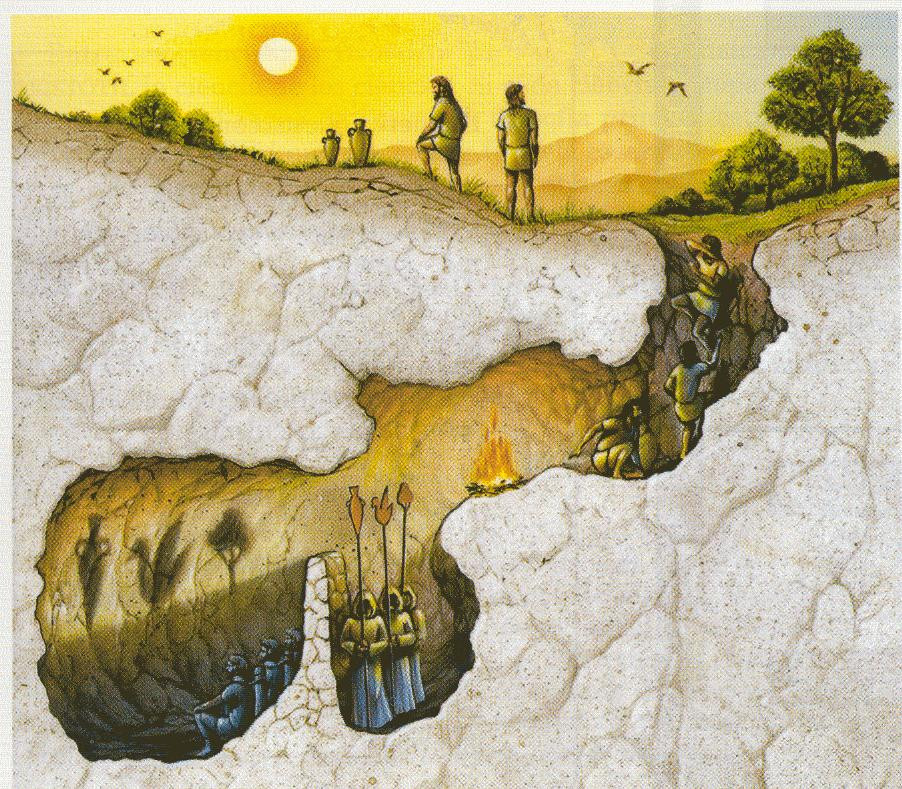
\includegraphics[width=0.5\textwidth]{figures/1-cave.jpg}
	\caption{Allégorie de la caverne. La célèbre histoire de
	Platon~\parencite{Platon} raconte l'histoire d'hommes condamnés à ne voir que
	l'apparence des phénomènes qui les entourent. Afin de parvenir à la connaissance de la réalité
	intelligible des Idées, ils doivent effectuer une démarche intellectuelle
	et sortir de la caverne.}\label{caverne}
\end{figure}


Les modèles les plus complets pour décrire un plasma sont sans
conteste les modèles cinétiques. Cependant, en plus d'être très coûteux à
résoudre numériquement, ces modèles donnent des résultats très bruités
et difficilement interprétables. Pour comprendre les phénomènes qui ont
lieu dans les plasmas, on leur préfère donc assez souvent les modèles fluides
plus simples et plus intuitifs.
En fonction des processus et des phénomènes de transport que l'on désire
observer, les modèles fluides permettent d'isoler, de négliger, ou même d'amplifier certains
termes, et sont donc plus à même de nous aider à comprendre les liens entre les
différents mécanismes.

Dans la théorie fluide, l'équation de quantité de
mouvement \eqref{1-eqMouvement}, qui contrôle l'évolution des vitesses fluides
$\mathbf u_\alpha$, régit l'essentiel de la dynamique du plasma. Cependant, sa forme complète
 est encore trop compliquée, et il est courant de la
simplifier davantage en considérant certaines approximations.

La première hypothèse communément retenue dans le domaine des
plasmas froids pour simplifier l'équation de la quantité de mouvement consiste à considérer le
tenseur de pression isotrope, i.e.
$\boldsymbol{\Pi}_\alpha=0$, en supposant que les transferts d'impulsion dus
aux collisions entre particules d'espèces différentes ont plus d'effet que
ceux résultants de la viscosité\footnote{Cette approximation s'applique en
général aux fluides dont la vitesse est de l'ordre de la vitesse sonique et
pour lesquels les termes de pression sont négligeables.
Dans le domaine des plasmas totalement ionisés, on utilise cette
approximation dans les limites MHD et plasmas froids ($T_i\sim\,$0) des
équations de Braginsky~\parencite{Fitzpatrick}. Elle n'est cependant plus valide
pour décrire les plasmas dont la vitesse caractéristique est lente devant la
vitesse thermique (c'est typiquement le cas des plasmas de bord des tokamaks,
où la vitesse fluide perpendiculaire est une vitesse de dérive de plusieurs
ordre de grandeur inférieure à la vitesse thermique).}.
L'équation de la quantité de mouvement~\eqref{1-eqMouvement} se réduit ainsi à un équilibre entre les forces
d'inertie, de frottement, de Lorentz et de pression :

\begin{equation}
\label{1-eqBilanForce}
\underbrace{m_\alpha \left(\partial_t \mathbf{u_\alpha} +
(\mathbf{u_\alpha}\cdot\nabla)\mathbf{u_\alpha}\right)}_\text{Inertie}
+\underbrace{m_\alpha\left(\nu_\alpha^c+
\nu_\alpha^\text{iz}\right)\mathbf
u_\alpha}_\text{Frottement \& Création}=\underbrace{{q_\alpha}\left(\mathbf
E+\mathbf u_\alpha\times \mathbf B\right)}_\text{Forces électromagnétiques}
-\underbrace{\frac{\nabla p_\alpha}{n_\alpha}}_\text{Pression}
\end{equation}
 
Le poids des différents termes de \eqref{1-eqBilanForce} varie en fonction des
paramètres du plasma et permet de définir les types de mécanismes qui régissent
le transport des fluides électroniques et ioniques. Les termes estimés petits
relativement aux autres peuvent ainsi être négligés pour obtenir une
expression plus simple de la vitesse fluide et permettre des développements
analytiques.

Un premier cas limite peut être obtenu en l'absence de champ magnétique quand
le terme de pression domine sur l'ensemble des termes du membre de gauche de
\eqref{1-eqBilanForce}. Ce cas de figure est caractéristique pour des électrons
non-collisionnels enfermés dans un puit de potentiel (par exemple résultant de
l'interaction entre le plasma et les parois). Dans ces conditions, le champ électrique et le gradient
de pression se compensent, et \eqref{1-eqBilanForce} s'écrit:

\begin{equation}
\label{1-equilibreBoltzman}
-e\mathbf
E =\frac{\nabla (n_e T_e)}{n_e}
\end{equation}

C'est la relation de Boltzmann, qui peut aussi s'obtenir naturellement en
intégrant la distribution de Boltzmann :

\begin{equation}
\label{1-profilBoltzman}
n_e=n_0\exp(\frac{e\Phi}{T_e})
\end{equation}

Cette hypothèse est fondamentale dans la dérivation des modèles fluides
de transport pour les plasmas dans la mesure où elle constitue l'une des bases
de la théorie des gaines vue précédemment.
En présence d'un champ magnétique,
\eqref{1-equilibreBoltzman} est une approximation souvent utilisée pour
décrire la direction parallèle aux lignes de champ. 

Dans le domaine des plasmas de fusion fortement magnétisés, il est
d'usage de considérer le petit paramètre $\delta=\rho_L/L$ pour moyenner
l'équation \eqref{1-eqBilanForce} sur les échelles de temps supérieures à
l'inverse de la fréquence cyclotronique $\omega_{c}$.
Dans le domaine des plasmas
froids, on fait plutôt l'hypothèse de forte collisionnalité et on développe
l'équation de la quantité de mouvement en fonction du petit paramètre
$\lambda/L$.

\section{Approche par les vitesses de dérive}
\label{vitessesDerive}
L'approche par les vitesses de dérive est à la base de nombreux modèles
développés pour étudier le transport dans les plasmas de fusion par
confinement magnétique\footnote{pour plus de détails sur la fusion par
confinement magnétique et les tokamaks, voir
l'annexe~\ref{AnnexeA}}~\parencite{Garcia,Bisai,Tamain}. Dans cette approche, la vitesse des particules est exprimée en fonction du mouvement cyclotronique rapide, d'une composante
parallèle au champ magnétique et d'une dérive lente du centre-guide des particules dans
la direction transverse. Cette décomposition, qui peut se voir comme une
version fluide de la théorie particulaire du centre-guide, sous-entend que les
fréquences cyclotroniques et les rayons de Larmor sont respectivement grandes
et petits devant les échelles caractéristiques du transport, i.e. :

\begin{equation}
\omega_{ce},\omega_{ci}\gg\omega\;\;\;\;\;\;\;\;\;\text{et}\;\;\;\;\;\;\;\;\;\rho_{Le},\rho_{Li}\ll
L_\nabla \end{equation} 

$L_\nabla$ étant la longueur de gradient caractéristique du
plasma dans la direction perpendiculaire au champ magnéique. 
 
\subsection{Les plasmas de la Scrape-Off-Layer}
La Scrape-Off-Layer des tokamaks, ou SOL, est la zone en périphérie du
plasma confiné, i.e.
qui commence à partir de la séparatrice et qui peut éventuellement s'étendre jusqu'aux parois internes du tore (voir
figure~\ref{SOL}). Dans cette région, les
particules ne sont plus confinées car les lignes de champ interceptent un
obstacle matériel (un limiteur ou un divertor) traité et dessiné spécifiquement
pour supporter les flux de matière et de chaleur qui s'échappent du plasma de
c\oe ur par transport transverse.
En conséquence, les profils de densité et de température s'effondrent sur une
longueur caractéristique qui définit la largeur de la SOL, $\lambda_\text{SOL}$,
donnant naissance à de forts gradients qui maintiennent le plasma hors
de l'équilibre thermodynamique.

\begin{figure}[!htbp]
    \centering
	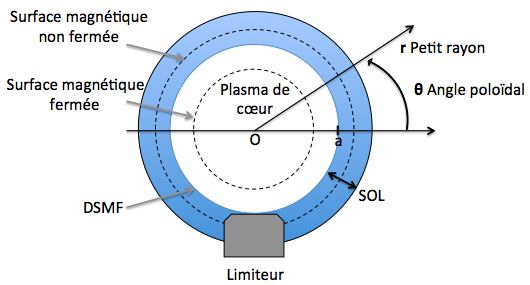
\includegraphics[width=0.8\textwidth]{figures/1-SOLLimiter.png}
	\caption{Coupe poloïdale du tokamak en configuration limiteur. De part et
	d'autre de la Dernière Surface Magnétique Fermée (DSMF située en r=a), le
	limiteur sépare le plasma de c\oe ur (r<a) de la SOL (r>a).}\label{SOL}
\end{figure}
 
Typiquement, les plasmas de SOL ont une densité de
l'ordre de 10$^{19}$~m$^{-3}$ et une température inférieure à la centaine
d'électronvolts. À cette température, le plasma est presque totalement ionisé et
le champ magnétique, de plusieurs Teslas, confine efficacement les particules
dans un mouvement cyclotronique de fréquence
$\omega_{c\alpha}=|q_\alpha|B/m_\alpha$. Pour un champ magnétique de 3~Teslas,
typique des tokamaks, ces fréquences sont de l'ordre de
$\omega_{ci}\sim\,$50~MHz pour un proton et de $\omega_{ce}\sim\,$80~GHz pour un électron.
Elles sont toutes deux bien supérieures à la fréquence caractéristique du
transport parallèle :

\begin{equation}
\omega_\para\sim
\frac{v_{{T}_\alpha}}{L_\para}\approx\omega_{c\alpha}\frac{\rho_{L\alpha}}{L_\para}\rightarrow
\delta=\frac{\rho_{L\alpha}}{L_\para}=\frac{\omega_\para}{\omega_{c\alpha}}\ll1
\end{equation} 

Dans la direction perpendiculaire au champ
magnétique, les vitesses de dérive
\mbox{(cf.~\S~\ref{Introduction}-\ref{1-plasma-champMag})} associées aux
gradients transverses entraînent un
transport de fréquence caractéristique $\omega_\perp$ de deux
ordres de grandeur inférieur à $\omega_{c\alpha}$\footnote{Les longueurs de
gradient typiques $L_\nabla$, de quelques centimètres, sont d'au moins un ordre
de grandeur supérieures aux rayons de Larmor ionique et électronique ($\rho_{Li}\approx3.10^{-4}$~m et
$\rho_{Le}\approx7.10^{-6}$~m pour une température de 70~eV et un champ
magnétique de 3~T). La fréquence caractéristique du transport perpendiculaire
est alors de l'ordre de la vitesse caractérisque transverse $v_\perp\sim
v_{{T}_\alpha}\rho_{L\alpha}/L_\nabla$ sur la longueur de corrélation $L_\para$
du plasma~\parencite{SarazinPhD} : $$\omega_\perp\sim v_\perp/L_\para\sim\rho_{L\alpha} v_{{T}_\alpha}/(L_\para L_\nabla)$$} :

\begin{equation}
\frac{\omega_\perp}{\omega_{c\alpha}}\approx \delta^2
\end{equation}

Malgré leur faible fréquence, ces vitesses de dérives sont à l'origine de tous
les mécanismes de micro-turbulence et jouent ainsi un rôle primordial dans le
problème du confinement des plasmas de fusion.

\subsection{Vitesses de dérive électrique et diamagnétique}

Quand le degré d'ionisation du plasma est très élevé, le terme issu de
l'interaction avec le gaz peut être négligé dans l'équation de la quantité de
mouvement~\eqref{1-eqBilanForce} :

\begin{equation}
\label{1-eqSOL}
 m_\alpha n_\alpha\left(\partial_t \mathbf{u_\alpha} +
(\mathbf{u_\alpha}\cdot\nabla)\mathbf{u_\alpha}\right)
={q_\alpha n_\alpha}\left(\mathbf E+\mathbf
u_\alpha\times \mathbf B\right)
-{\nabla p_\alpha}
\end{equation}

 Sous l'hypothèse de faible variation spatiale des grandeurs et des champs à
 l'échelle du rayon de Larmor, la lente évolution du système par rapport aux
 fréquences cyclotroniques permet d'effectuer un développement de la vitesse
 perpendiculaire $\mathbf u_{\alpha\perp}$ en fonction du petit paramètre
 $\varepsilon_\omega=\omega/\omega_{c}$ :
 
 \begin{equation}
 \label{2-developEqMvt}
 \mathbf u_{\alpha\perp}=\mathbf
 u_{\alpha\perp}^{(0)}+\epsilon_\omega \mathbf
 u_{\alpha\perp}^{(1)}+\epsilon^2_\omega \mathbf u_{\alpha\perp}^{(2)}+\ldots
 \end{equation}
 
 En négligeant le mouvement cyclotronique, qui correspond à l'ordre 0 de ce développement et qui
 est de moyenne nulle sur un temps $t\sim\omega_{c\alpha}^{-1}$, la projection
 de~\eqref{1-eqSOL} perpendiculairement au champ magnétique s'écrit à l'ordre 1
 en $\varepsilon_\omega$ :
 
 \begin{equation}
\label{1-eqSOLperp}
0
={q_\alpha n_\alpha}\left(\mathbf E+\mathbf
u_{\alpha\perp}^{(1)}\times \mathbf B\right)
-{\nabla_\perp p_\alpha}
\end{equation}

où $\mathbf E$ est le champ électrique dérivant du potentiel électrostatique
$\Phi$. En prenant le produit vectoriel par $\mathbf B$ de cette équation, on
obtient les deux vitesses de dérive fluides principales, la vitesse de dérive
électrique $\mathbf u_E$ et la vitesse de dérive diamagnétique $\mathbf
u^\alpha_*$, respectivement liées aux gradients transverses de potentiel
électrique $\Phi$ et de pression $p_\alpha$:

\begin{equation}
\label{1-eqVitessesDerive}
\mathbf u_{\alpha\perp}^{(1)}=\mathbf u_E+\mathbf u^\alpha_*=\frac{\mathbf
B\times\nabla_\perp \Phi}{B^2}+\frac{\mathbf B\times\nabla_\perp
p_\alpha}{n_\alpha q_\alpha B^2}
\end{equation}

\begin{figure}[!htbp]
    \centering
	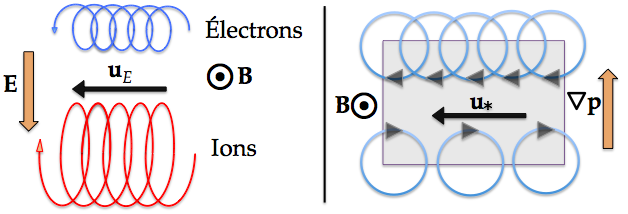
\includegraphics[width=0.9\textwidth]{figures/1-vitessesDerive.png}
	\caption{Schémas des vitesses de dérive électrique (à gauche) et diamagnétique
	(à droite).}
	\label{1-vitessesDerive}
\end{figure}

L'origine de ces vitesses de dérive est illustrée sur la
figure~\ref{1-vitessesDerive}. La dérive électrique provient de l'accumulation
de petites déviations du mouvement cyclotronique, tantôt accéléré et tantôt
ralenti par le champ électrique. La dérive diamagnétique est une vitesse
purement fluide qui traduit le mouvement d'ensemble des particules, et non une
dérive individuelle de celles-ci. De ce fait, elle ne transporte que très peu
de matière en comparaison de la dérive électrique : pour s'en convaincre, il
suffit de regarder la divergence des flux issus de ces vitesses :

\begin{equation}
\label{1-divElecDrift}
\begin{split}
\nabla\cdot\left(n_\alpha\mathbf
u_E\right)&=\nabla\cdot\left(n_\alpha\frac{\mathbf B\times\nabla
\Phi}{B^2}\right) =\nabla \Phi\times\nabla\frac{n_\alpha}{B}\cdot \mathbf b\\
&=\frac{\nabla \Phi}{\mathbf B}\times\nabla n_\alpha\cdot \mathbf
b+\underbrace{n_\alpha\nabla
\Phi\times\nabla\frac{1}{B}\cdot \mathbf b}_{\text{terme de
courbure}\;\propto\nabla 1/B}
\end{split}
\end{equation}

\begin{equation}
\nabla\cdot\left(n_\alpha\mathbf
u^\alpha_*\right)=\nabla\cdot\left(\frac{\mathbf B\times\nabla
p_\alpha}{q_\alpha B^2}\right)
=\underbrace{\frac{1}{q_\alpha}\nabla
p_\alpha\times\nabla\frac{1}{B}\cdot \mathbf b}_{\text{terme de
courbure}\;\propto\nabla 1/B}
\end{equation}

L'intensité du champ magnétique varie très peu dans la SOL. Les fluctuations de
potentiel électrique $\widetilde{\Phi}$ et de densité $\widetilde{n}$
sont de plusieurs ordres de grandeurs supérieures à celles du champ magnétique
radial $B_r$ : $\widetilde{n}$/$n$ peut atteindre la valeur 1 proche de la
paroi, tandis que $\widetilde{B}_r$/$B$ ne dépasse guère
10$^{-4}$~\parencite{SarazinPhD}.
On peut ainsi négliger les effets de courbure et ne considérer que l'avection par
la dérive électrique dans la divergence du flux~\eqref{1-divElecDrift} :
$\nabla\cdot(n_\alpha\mathbf u_E)\approx \mathbf u_E\cdot\nabla n$. La divergence du flux diamagnétique, qui
n'est due qu'aux effets de courbure du champ magnétique, est très faible, voir
nulle dans le cas d'un champ magnétique uniforme $\nabla1/B\,$=~0.
Par contre, et comme précisé au paragraphe \S~\ref{1-plasma-champMag}, la dérive
diamagnétique est sensible à la charge des particules et est donc la seule à porter du courant.
L'influence de ce courant est fondamentale dans la stabilité du plasma :

\begin{equation}
\mathbf j_*=(q_in_i\mathbf u^i_*-q_en_e\mathbf
u^e_*)=\nabla(p_i+p_e)\times\mathbf B/B^2
\end{equation}



\subsection{Dérive de polarisation}

Pour obtenir la vitesse de dérive au second ordre, nous reconsidérons
l'équation de conservation de la quantité de mouvement~\eqref{1-eqBilanForce}
dans le cadre du développement \eqref{2-developEqMvt}. Si on
ne garde que les termes à l'ordre~2, qui contiennent les dérives à l'ordre~1
dans le terme intertiel\footnote{\label{2-footnoteBraginsky}Théoriquement, il faut aussi
tenir compte de la divergence du tenseur de pression de Braginsky
$-\nabla\cdot\boldsymbol{\pi}^{(1)}_\alpha$ et du terme de issu des collisions
coulombiennes $\mathbf R_{ei}$. Cependant ces termes
n'interviennent qu'à l'ordre 2 en
$\varepsilon_\omega$ du développement de $\mathbf u_{\alpha\perp}$ et on peut
montrer que leur principale contribution est de compenser les termes inertiels
d'advection par la dérive diamagnétique~\parencite{Tamain2}. Tous ces termes
disparaissent donc de l'expression finale de la dérive de polarisation et
nous les omettons pour des raisons de simplicité.}, on aboutit à :

\begin{equation}
m_\alpha n_\alpha\left[\partial_t \mathbf{u}^{(1)}_{\alpha\perp} +
\left((\mathbf{u}_{\alpha\para}+\mathbf
u^{(1)}_{\alpha\perp})\cdot\nabla\right)\mathbf{u}^{(1)}_{\alpha\perp}\right]
=n_\alpha q_\alpha\mathbf u^{(2)}_{\alpha\perp}\times \mathbf
B
\end{equation}

En insérant l'expression des vitesses de dérive à l'ordre 1, et en ne tenant pas
compte de l'advection par la vitesse diamagnétique (voir
note$^\text{\ref{2-footnoteBraginsky}}$) la dérive d'ordre 2 s'écrit :

\begin{equation}
\label{1-vitessePol2}
\mathbf{u}_{\alpha\perp}^{(2)}\approx\frac{m_\alpha}{q_\alpha
B^2}\mathbf
B\times\left(\frac{\partial}{\partial{t}}+(\mathbf
u_{\alpha\para}+\mathbf u_{E})\cdot\nabla\right)(\mathbf u_E +
\mathbf u^\alpha_*)
\end{equation}

C'est la dérive de polarisation $\mathbf{u}_{\alpha\perp}^{(2)}=\mathbf
u^\alpha_p$, qui dérive du terme d'inertie. 
La présence du ratio $m_\alpha/q_\alpha$ indique
d'une part que cette vitesse porte du courant, et d'autre part que ce
courant est principalement porté par les ions $\mathbf{j}_p\approx en_i\mathbf
u^i_p$. En faisant de plus l'hypothèse des ions froids, la divergence de la vitesse de dérive diamagnétique peut être
négligée dans~\eqref{1-vitessePol2}, et le courant s'écrit:

\begin{equation}
\label{1-courantPol}
\mathbf{j}_p \approx-\frac{en_im_i}{q_i
B^2}\mathbf B\times\frac{\text{d}\mathbf u_E}{\text{dt}}=
-\frac{en_im_i}{q_i B^2}\frac{\text{d}\nabla_\perp \Phi}{\text{dt}}
\end{equation}

avec la dérivée totale $d/dt=\partial/\partial t + (\mathbf
u_{\alpha\para}+\mathbf u_{E})\cdot\nabla$. Bien que la vitesse de
polarisation soit d'un ordre de grandeur inférieur aux deux autres vitesses de dérive, la divergence du flux 
de polarisation est comparable à celle du flux diamagnétique. Comme
la dérive électrique ne transporte aucun courant, la
contribution de la dérive de polarisation dans
l'équation du courant est dès lors du même ordre de
grandeur que celle de la dérive diamagnétique (du fait que celle-ci ne
transporte qu'aux effets de courbure près) et ne peut plus être négligée.

\section{Cas collisionnel : Équation de Dérive-Diffusion}
\label{1-transportAmbipolaire}
\subsection{Équation de Dérive-Diffusion non magnétisée}
Les plasmas froids de décharge utilisés dans l'industrie et la recherche n'ont
en général qu'un faible degré d'ionisation $\alpha<$1\% et la dynamique des
espèces y est dominée par la perte de quantité de mouvement liée à l'ionisation
et aux collisions avec le gaz. Pour modéliser ce type de plasma, la prise en
compte du terme collisionnel dans l'équation de la quantité de mouvement est
essentielle. 


En l'absence de champ magnétique, le rapport d'échelle entre le libre parcours moyen des particules
et la taille du plasma $\lambda_\alpha\ll L$ permet ensuite de simplifier
l'équation de la quantité de mouvement en négligeant les termes d'inertie, relativement
faibles par rapport au terme collisionnel :

\begin{equation}
\label{1-eqDriftDif}
n_\alpha\mathbf u_\alpha=\frac{q_\alpha}{\nu_\alpha m_\alpha}n_\alpha\mathbf
E-\frac{\nabla\left(n_\alpha T_\alpha\right)}{\nu_\alpha
m_\alpha}
\end{equation}

avec $\nu_\alpha=\nu_\alpha^c+\nu_\alpha^\text{iz}$ une fréquence de collision
effective. Dans le cas d'un plasma isotherme, on peut sortir la température de
la divergence.
En notant $\mu_\alpha=|q_\alpha|/\nu_\alpha m_\alpha$ et
$D_\alpha=T_\alpha/\nu_\alpha m_\alpha$, le flux de \eqref{1-eqDriftDif} se
réécrit avec une loi d'Ohm et une loi de Fick :

\begin{equation}
\label{1-eqDriftDif2}
n_\alpha\mathbf u_\alpha\equiv\underbrace{\frac{q_\alpha}{|q_\alpha|}\mu_\alpha n_\alpha\mathbf E}_\text{Loi d'Ohm}+\underbrace{D_\alpha{\nabla n_\alpha}}_\text{Loi
de Fick}
\end{equation}

 C'est le flux de Dérive-Diffusion, caractérisé par les coefficients de
transport $\mu_\alpha$ et
$D_\alpha$, tous deux inversement proportionnels à la fréquence de collision
$\nu_\alpha$ (donc à la densité de gaz), et reliés par la relation d'Einstein :

\begin{equation}
\label{1-EinsteinRelation}
D_\alpha/\mu_\alpha=\frac{T_\alpha}{|q_\alpha|}
\end{equation}

\begin{itemize}
  \item la mobilité, définie par $\mu_\alpha$,
  mesure la disposition d'une espèce à laisser passer le courant au sein d'un
  milieu ; 
  \item la diffusion, de coefficient $D_\alpha$,
  représente la tendance naturelle d'un système à rendre homogène sa densité de particule sous l'effet
  de l'agitation thermique.
\end{itemize}

En combinant \eqref{1-eqDriftDif2} avec l'équation de continuité
\eqref{1-eqContinuite}, on obtient l'équation d'évolution de la densité
dite de Dérive-Diffusion :
 
\begin{equation}
\label{1-eqDriftDifContinuite}
\partial_t
n_\alpha=\nabla\cdot({\frac{q_\alpha}{|q_\alpha|}\mu_\alpha n_\alpha\mathbf E}
+{D_\alpha{\nabla n_\alpha}})+S_\alpha
\end{equation}

Dans des plasmas de décharge collisionnels, à partir de la source d'ionisation,
les électrons ont tendance à se déplacer beaucoup plus rapidement que les ions
du fait de leur faible masse et de leur température. Cette différence de
mobilité entraîne l'apparition d'un champ électrique dit "ambipolaire"
$\mathbf E_a$, faisant dériver les ions et les électrons ensembles et
systématiquement dirigé dans le sens opposé du gradient de densité afin de
limiter la diffusion des électrons et accélérer les ions. En ne considérant
qu'une seule espèce ionique, on trouve son expression en cherchant le champ
correspondant à un courant nul :
 
\begin{equation}
\label{1-eqEAmb}
\mathbf j=0 \Rightarrow \mathbf E=\mathbf
E_a=\frac{D_i-D_e}{\mu_i+\mu_e}\frac{\nabla
n}{n}
\end{equation}

Si l'on applique l'équation de
Dérive-Diffusion~\eqref{1-eqDriftDifContinuite} à un plasma peu collisionnel,
i.e. dans la limite $\nu_{i,e}\rightarrow\,$0, cette description peut poser
problème, les mobilités tendant quant à elles vers l'infini. Le modèle de
Dérive-Diffusion n'est en effet strictement valide que quand le libre parcours
moyen ne dépasse pas la longueur caractéristique des gradients $\lambda\le
L_{\nabla}$.

Quand ce critère n'est pas respecté, cela importe peu pour les
électrons, l'équilibre de
Boltzmann tenant toujours.
Pour les ions, la seule issue repose sur la prise en compte du
terme de création $\nu^\text{iz}_i\mathbf u_i$ qui défini une limite haute pour
la mobilité ionique.
Le modèle de Dérive-Diffusion est ainsi encore utilisable, mais perd beaucoup en
précision.

Regardons maintenant ce que donne ce modèle en présence d'un champ magnétique.

\subsection{Équation de Dérive-Diffusion magnétisée}
\label{1-deriveDiffMag}
L'utilisation d'un champ magnétique dans un plasma permet de contrôler en partie
le transport des particules et d'obtenir des configurations favorables pour
diverses applications. Cependant, la prise en compte du terme de Laplace dans
\eqref{1-eqBilanForce} impose une forte anisotropie dans le système, ce qui
complexifie considérablement les phénomènes de transport. En
négligeant l'inertie, on peut considérer \eqref{1-eqBilanForce} comme une
équation algébrique d'inconnue $\mathbf u$ ; le réagencement des différents
termes donne :

\begin{equation}
\label{2-eqDriftDifMag}
\begin{split}
n_\alpha\mathbf u_\alpha&=\frac{q_\alpha}{|q_\alpha|}\mu_\alpha
n_\alpha\left(\mathbf E+\mathbf u_\alpha\times\mathbf
B\right)-D_\alpha\nabla\left( n_\alpha\right)
\\
&=\frac{q_\alpha}{|q_\alpha|} n_\alpha\left(\mu_{\alpha_\para}\left(\mathbf
b\cdot\mathbf E\right)\mathbf b+\mu_{\alpha_\perp}\left(\mathbf
E-\left(\mathbf
b\cdot\mathbf E\right)\mathbf
b\right)+\mu_{\alpha_\times}\mathbf
b\times\mathbf E\right)
\\
&-\left(D_{\alpha_\para}\left(\mathbf
b\cdot\nabla n_\alpha\right)\mathbf b+D_{\alpha_\perp}\left(\mathbf
\nabla n_\alpha-\left(\mathbf
b\cdot\nabla n_\alpha\right)\mathbf
b\right)+D_{\alpha_\times}\mathbf
b\times\mathbf \nabla n_\alpha\right)
\end{split}
\end{equation}

Pour une meilleure lisibilité, on réécrit l'équation~\ref{2-eqDriftDifMag}
sous forme tensorielle, donnant l'équation de Dérive-Diffusion magnétisée,
couramment utilisée dans le domaine des plasmas froids pour modéliser le
transport magnétisé~\parencite{HagelaarDeriveDiff, HagelaarProp} :

\begin{equation}
\label{2-eqDriftDifMag2}
n_\alpha\mathbf u_\alpha\equiv
\frac{q_\alpha}{|q_\alpha|} n_\alpha\boldsymbol{\mu}_\alpha\cdot \mathbf
E-\mathbf{D}_\alpha{\nabla\left( n_\alpha\right)}
\end{equation}

où la mobilité $\boldsymbol{\mu}_\alpha$ et la diffusion $\mathbf{D}_\alpha$
sont devenus des tenseurs d'ordre 2. Dans un repère avec le champ magnétique axé
sur la direction du champ magnétique $\mathbf B=B\mathbf e_z$ :

\begin{align}
\boldsymbol{\mu}_\alpha =
 \begin{pmatrix}
  \mu_{\alpha_\perp} & \pm\mu_{\alpha_\times} & 0 \\
  \pm\mu_{\alpha_\times} & \mu_{\alpha_\perp} & 0 \\
  0  & 0  & \mu_{\alpha_\para} 
 \end{pmatrix}\;\;\;\;\text{et}\;\;\;\;
 \mathbf D_\alpha =
 \begin{pmatrix}
  D_{\alpha_\perp} & \pm D_{\alpha_\times} & 0 \\
 \pm D_{\alpha_\times} & D_{\alpha_\perp} & 0 \\
  0  & 0  & D_{\alpha_\para} 
 \end{pmatrix}
\end{align}

Dans la direction parallèle au champ magnétique, les coefficients de mobilité et
de diffusion sont inchangés
$\mu_{\alpha\para}=\mu_{\alpha}=|q_\alpha|/m_\alpha\nu_\alpha$ et
$D_{\alpha\para}=D_\alpha=T_\alpha/m_\alpha\nu_\alpha$. Les coefficients de la
direction perpendiculaire font quant à eux apparaître le paramètre de Hall
$h_\alpha=eB/m_\alpha\nu_\alpha$ :

\begin{align}
\mu_{\alpha\perp}=\frac{1}{1+h_\alpha^2}\mu_\alpha\;\;\;\;\;\;\;\;
\;\;\;\;D_{\alpha\perp}=\frac{1}{1+h_\alpha^2}D_\alpha
\end{align}
\begin{align}
\mu_{\alpha\times}=\frac{h_\alpha}{1+h_\alpha^2}\mu_\alpha\;\;\;\;
\;\;\;\;\;\;\;\;D_{\alpha\times}=\frac{h_\alpha}{1+h_\alpha^2}D_\alpha
\end{align}

Quand $h_\alpha=0$, les tenseurs sont diagonaux et isotropes. Ensuite, plus le
paramètre de Hall augmente, plus le transport dans les directions transverses se
réduit :
les coefficients indicés avec le symbole perpendiculaire sont inversement
proportionnels au carré du champ magnétique $\mu_{\alpha\perp},
D_{\alpha\perp}\propto B\puissance{-2}$ ; à partir de $h_\alpha=1$, le
transport croisé commence à dominer sur le transport collisionnel et devient proportionnel à
$B\puissance{-1}$. Cette loi de puissance que suit le transport par rapport au
champ magnétique est souvent interprétée comme la signature d'un transport
anormal, mais apparaît naturellement dans les équations à travers les
coefficients de transport $\mu_{\alpha\times}$ et $D_{\alpha\times}$.

Dans les sources magnétisées, pour un paramètre de Hall électronique de l'ordre
de $h_e\approx\,$1000, on obtient typiquement des ratios sur les mobilités :

\begin{equation}
\frac{\mu_{e_\perp}}{\mu_{e_\para}}\approx
10^{-6}-10^{-10}\text{~~~~~~~~et~~~~~~~~}\frac{\mu_{e_\times}}{\mu_{e_\para}}\approx
\frac{\mu_{e_\perp}}{\mu_{e_\times}}\approx10^{-3}
\end{equation}

En revanche, les ions n'étant généralement que peu magnétisés, leur mobilité
dans la direction perpendiculaire reste principalement fonction de la fréquence
de collision et d'ionisation  :

\begin{align}
\mu_{i_\perp}&=\frac{1}{1+h_i^2}\mu_i=\frac{q_i\nu_i}{m_i(\nu_i^2+\omega_{ci}^2)}\propto\frac{1}{\nu_i}\\
\mu_{i_\times}&=\frac{h_i}{1+h_i^2}\mu_i=\frac{q_i^2B}{m_i^2(\nu_i^2+\omega_{ci}^2)}\propto\frac{B}{\nu_i^2}
\end{align}

À travers le champ magnétique, les ions sont alors plus rapides que les
électrons, les deux fluides se séparent, entraînant l'apparition de
courants. Ce sont les courants perpendiculaires de Pedersen et de Hall :

\begin{align}
\mathbf j_{\perp\text{Ped}}&=en\left((\mu_{i\perp}+\mu_{e\perp})\mathbf E_\perp
- (D_{i\perp}-D_{e\perp})\frac{\nabla_\perp n}{n}\right)\\
\mathbf j_{\perp\text{Hall}}&=en\left((\mu_{e\times}-\mu_{i\times})\mathbf
b\times\mathbf E_\perp - (D_{e\times}-D_{i\times})\mathbf
b\times\frac{\nabla_\perp n}{n}\right)
\end{align}

Au fur et à mesure de l'ionisation du gaz $\nu_e, \nu_i\rightarrow\,$0. Les
coefficients de transport correspondants se simplifient :

\begin{align}
\mu_{\alpha\perp}&=\frac{1}{1+h_\alpha^2}\mu_\alpha=\frac{|q_alpha|\nu_\alpha}{m_\alpha(\nu_\alpha^2+\omega_{c\alpha}^2)}\rightarrow
0 &D_{\alpha\perp}=\frac{1}{1+h_\alpha^2}D_\alpha\rightarrow 0
\\
\mu_{\alpha\times}&=\frac{h_\alpha}{1+h_\alpha^2}\mu_\alpha=\frac{|q_alpha\omega_{c\alpha}|}{m_\alpha(\nu_\alpha^2+\omega_{c\alpha}^2)}\rightarrow\frac{1}{B}
&D_{\alpha\times}=\frac{h_\alpha}{1+h_\alpha^2}D_\alpha\rightarrow\frac{T_\alpha}{q_\alpha
B}
\end{align}

On retrouve alors les vitesses de dérive électrique et diamagnétique
introduites dans la partie précédente :

\begin{equation}
\begin{split}
\mathbf u_\alpha&=\frac{q_\alpha}{|q_\alpha|}\boldsymbol{\mu}_\alpha
\mathbf E-\mathbf D_\alpha\frac{\nabla\left( n_\alpha\right)}{n_\alpha}
\\
&= \frac{q_\alpha}{|q_\alpha|}\mu_{\alpha_\para} E_\para -
D_{\alpha\para}\frac{\nabla_\para n_\alpha}{n_\alpha} + \frac{\mathbf
B\times\nabla_\perp \Phi}{B^2}+\frac{T_\alpha\mathbf B\times\nabla_\perp
n_\alpha}{n_\alpha q_\alpha B^2}
\end{split}
\end{equation}

\section{Discussion}
Nous avons présenté deux modèles respectivement utilisés dans le domaines des
plasmas de fusion et des plasmas froids et allons maintenant discuter de leur
pertinence pour décrire une source basse-pression magnétisée.

\subsection{Sur le modèle des vitesses de dérive}
Le modèle basé sur les vitesses de dérive s'appuie sur de nombreuses
hypothèses et appoximations qui sont fondamentalement injustifiée dans le cadre
des sources :

\begin{itemize}
  \item Tout d'abord, le modèle considère un plasma totalement ionisé, ne tenant
  pas compte de l'interaction avec le gaz. Or, les collisions élastiques et
  inélastiques sont des éléments primordiaux dans la physique des plasmas froids. L'ionisation contrôle
  notamment le bilan de particule et c'est un puit de quantité de mouvement
  pouvant influencer fortement la dynamique ionique à basse pression de gaz.
  \item En l'absence de collision avec le gaz, la dérive électrique ne porte pas
  de courant et le champ électrique n'intervient dans l'équation du courant qu'à
  travers la vitesse de polarisation. Ce n'est pas vrai dans le cas des sources
  d'ions où elle est à l'origine du courant de Hall.
  \item Le dernier point, mais peut être le plus critique, concerne l'hypothèse
  de forte magnétisation des particules, qui fonde l'ensemble du modèle et qui
  s'éffondre dans les régions faiblement magnétisées des sources. Elle est de
  plus injustifiée pour les ions en général, qui ne font qu'apercevoir le champ
  magnétique.
\end{itemize}

Cependant, dans le développement en ordre, le modèle des vitesses de
dérive ne fait pas directement d'approximations (sur le tenseur de pression, les
collisions coulombiennes et l'inertie). On voit par exemple que dans l'équation
du courant, la présence des termes d'inertie joue un rôle majeur à travers le
courant de polarisation qui referme l'équation du courant.

Le modèle des vitesses de dérive peut aussi être adapté à la présence d'un gaz
en incluant le terme de collision dans l'expression de la vitesse. Cependant, 
on ne sait plus trop à quoi correspond le petit paramètre $\epsilon_\omega$ ni
si un développement en ordres successifs de $\epsilon_\omega$ a encore 
un sens quelconque (l'approche des vitesses de dérive est basée sur la
superposition du mouvement de dérive et d'un mouvement rapide de moyenne nulle).

\subsection{Sur le modèle de Dérive-Diffusion}

Le modèle de Dérive-Diffusion, encore très utilisé dans le domaine des plasmas
froids, pose quant à lui des problèmes sur d'autres points :

\begin{itemize}
  \item L'hypothèse de forte collisionnalité n'est pas rigoureusement justifiée
  dans les plasmas froids basse-pression. Le libre-parcours moyen ionique
  $\lambda_i$ excède souvent les dimensions de la source. On peut alors se
  rattraper avec la relation de Boltzmann et la prise en compte de l'ionisation
  mais le modèle donne des solutions moins précises. Pour obtenir des
  simulation correctes, le terme inertiel d'advection doit être considéré dans
  l'équation de la quantité de mouvement.
  \item L'équation de Dérive-Diffusion, discrétisée spatialement sur un
	stencil à 9 points, mène à un système linéaire potentiellement mal conditionné
	quand les coefficients de transport croisé sont supérieurs aux
	coefficients perpendiculaires, i.e. en présence d'un fort champ magnétique. Le
	probème est numériquement instable et devient difficile à résoudre. 
	\item Enfin, le modèle néglige totalement l'inertie des particules dont dérive
	le courant de polarisation, crucial dans la description du transport fortement
	magnétisé. On manque ainsi tout l'aspect dynamique du transport. Le
	modèle, en cherchant une solution stationnaire à un problème fondamentalement
	instationnaire, est donc très peu adapté au transport fortement magnétisé.
\end{itemize}

Le modèle de Dérive-Diffusion tel que présenté dans ce chapitre fait
l'hypothèse d'un plasma isotherme, mais cette hypothèse est assez facile à
lever et ne nécessite que peu de modification sur les équations et les
coefficients de transport. La prise en compte des termes d'inertie demande en
revanche un nouveau formalisme pour la dérivation du modèle, qui ne décrit plus
uniquement le phénomène simple de dérive-diffusion.

%\bibliographystyle{apalike}
%\bibliography{biblio}
\end{refsection}

